\documentclass[11pt,a4paper]{ctexart}
\usepackage{geometry}
\usepackage{fancyhdr}
\usepackage{titlesec}
\usepackage{enumitem}
\usepackage{hyperref}
\usepackage{setspace}
\usepackage{ulem}
\usepackage{xcolor}
\usepackage{times}
\usepackage{graphicx}
\usepackage[absolute,overlay]{textpos}


% 页面设置
\geometry{margin=1.5cm}
\pagestyle{fancy}
\fancyhf{}
\renewcommand{\headrulewidth}{0pt}

% 标题格式设置
\titleformat{\section}{\Large\bfseries}{\thesection}{1em}{}
\titlespacing{\section}{0pt}{12pt}{6pt}

% 设置超链接颜色为黑色
\hypersetup{
    colorlinks=true,
    linkcolor=black,
    urlcolor=black,
    citecolor=black
}

% 开始文档
\begin{document}

% 标题部分
\begin{center}
    {\Huge\bfseries 刘哲宁\quad$|$\quad 在读 \quad$|$\quad 随时到岗}
\end{center}

% 个人照片
\begin{textblock*}{5cm}(17cm, 0.2cm) % 在页面左上角右移10cm,下移5cm处放置图片
    
\includegraphics[width=1in]{../assets/profile.jpg}
  \end{textblock*}

% 个人信息
\begin{center}
    {\songti 邮箱:}{\fontfamily{ptm}\selectfont \href{mailto:liuzhening_roeh@163.com}{liuzhening\_roeh@163.com}} \hspace{1em}
    {\songti 电话:}{\fontfamily{ptm}\selectfont \href{tel:+8618234357464}{+86 18234357464}} \hspace{1em}
    {\songti 微信:}{\fontfamily{ptm}\selectfont hyper\_vapor} \hspace{1em}
    {\songti 主页:}{\fontfamily{ptm}\selectfont \uline{\href{https://hyper-vapor.github.io}{点此预览}}}
\end{center}

\hrule
\vspace{1em}

% 教育背景
{\heiti 教育背景}
\vspace{0.5em}

\begin{tabular}{@{}p{0.08\textwidth}p{0.18\textwidth}p{0.28\textwidth}p{0.18\textwidth}@{}}
{\fangsong 学士} & {\fangsong 2019.09-2023.06} & {\fangsong 西南交通大学(211工程)} & {\fangsong 电子科学与技术} \\
{\fangsong 硕士} & {\fangsong 2024.09-2027.06} & {\fangsong 西南交通大学(211工程)} & {\fangsong 计算机技术} \\
\end{tabular}

\vspace{1em}
{\heiti 英语}

{\songti CET 4、CET 6、 IELTS 6.5}

\vspace{1em}
\hrule
\vspace{1em}

% 技术能力
{\heiti 技术能力}
\begin{itemize}[itemsep=0pt,parsep=0pt,topsep=0pt]
    \item {\songti 熟悉JavaScript / TypeScript ES6+语法糖、对Javascript事件循环、原型链、闭包等特性有深刻理解}
    \item {\songti 掌握React框架,理解组件化、状态管理、生命周期、Hooks、虚拟DOM、Diff算法等原理}
    \item {\songti 熟悉Vite / Next.js / Webpack等构建工具或脚手架、npm / pnpm / yarn 包管理器,有前端工程化思维}
    \item {\songti 使用过TailwindCSS / Scss / Css Modules等CSS预处理器,有CSS布局、动画、响应式设计经验}
    \item {\songti 熟悉Express.js / FastAPI / Flask / PostgresSQL等后端生态,结合Baas平台可构建全栈应用}
    \item {\songti 了解Agent / RAG / Prompt设计范式,参与过LLMs应用层开发}
\end{itemize}

\vspace{1em}
\hrule
\vspace{1em}

% 实习经历
{\heiti 实习经历}

{\heiti 北京 \quad$|$\quad PuppyAgent \quad$|$\quad 前端开发 / 大模型应用开发 \quad$|$\quad 2025.06-2025.09}

\begin{itemize}[itemsep=0pt,parsep=0pt,topsep=0pt]
    \item 负责PuppyAgent的Web端开发,包括前端页面设计、开发和维护。
    \item 负责PuppyAgent的大模型应用开发,包括大模型应用的开发和维护。
\end{itemize}

\vspace{1em}
\hrule
\vspace{1em}

% 项目经历
{\heiti 项目经历}

{\heiti Prodlens \quad$|$\quad 最新AI产品数据分析与评测 \quad$|$\quad \uline{\href{https://prodlens.hypervapor.cloud}{点此预览}} \quad$|$\quad \uline{\href{https://github.com/HYPERVAPOR/prodlens}{Github仓库}}

\begin{itemize}[itemsep=0pt,parsep=0pt,topsep=0pt]
    \item {\songti 负责Prodlens的Web端开发,包括前端页面设计、开发和维护。}
    \item {\songti 负责Prodlens的大模型应用开发,包括大模型应用的开发和维护。}
\end{itemize}

\vspace{1em}
\hrule
\vspace{1em}

% 贡献日历
{\heiti 贡献日历}

\begin{figure}[h]
    \centering
    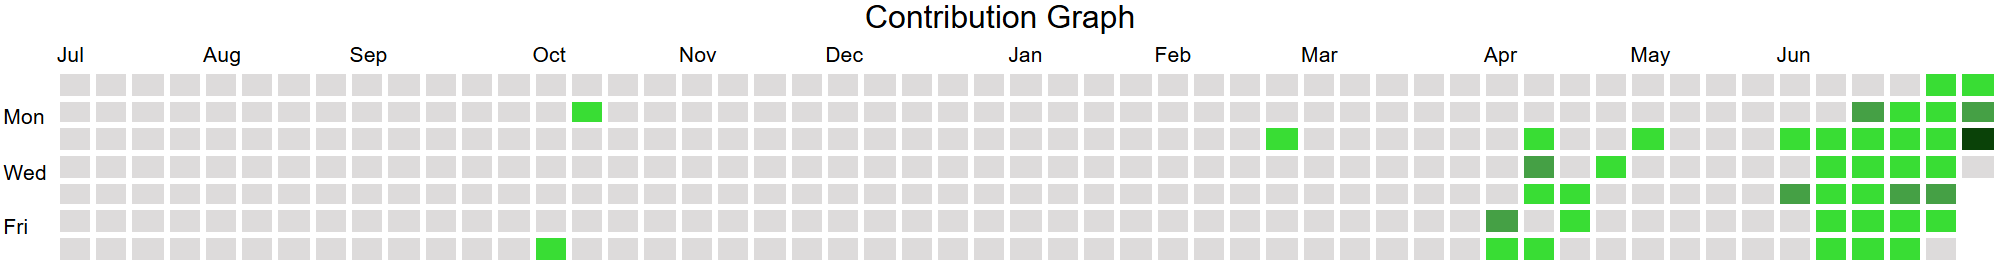
\includegraphics[width=0.8\textwidth]{../assets/github-contributions.png}
\end{figure}

\vspace{1em}
\hrule
\vspace{1em}

% 自我评价
{\heiti 自我评价}

\begin{itemize}[itemsep=0pt,parsep=0pt,topsep=0pt]
    \item {\songti 卓越的产品思维,能理解用户需求,并设计出优秀的产品}
    \item {\songti 熟悉基于看板和Git版本控制的团队协作开发流程,能快速响应需求变化}
    \item {\songti 可实习六个月及以上,不限地域}
\end{itemize}



\end{document}
